\documentclass[12pt, a4paper]{article}

% ── Packages ──────────────────────────────────────────────────────────────────
\usepackage[a4paper, margin=2.5cm]{geometry}
\usepackage{graphicx}
\usepackage{float}
\usepackage{amsmath}
\usepackage{amssymb}
\usepackage{xcolor}
\usepackage{mdframed}
\usepackage{parskip}
\usepackage{enumitem}
\usepackage{titlesec}
\usepackage{booktabs}
\usepackage{hyperref}
\usepackage[T1]{fontenc}
\usepackage[colorinlistoftodos]{todonotes}
\usepackage{listings}
\usepackage{courier}

% ── Graphics path ─────────────────────────────────────────────────────────────
\graphicspath{{../../Images_for_latex/Lecture_5/}}

% ── Colours ───────────────────────────────────────────────────────────────────
\definecolor{keyblue}{RGB}{30, 80, 160}
\definecolor{keybluebg}{RGB}{220, 235, 255}
\definecolor{noteorange}{RGB}{200, 100, 0}
\definecolor{noteorangebg}{RGB}{255, 240, 215}
\definecolor{warnred}{RGB}{180, 30, 30}
\definecolor{warnredbg}{RGB}{255, 220, 220}
\definecolor{defgreen}{RGB}{20, 110, 50}
\definecolor{defgreenbg}{RGB}{215, 245, 225}
\definecolor{headernavy}{RGB}{25, 35, 90}
\definecolor{codegray}{RGB}{245, 245, 245}
\definecolor{codecomment}{RGB}{100, 100, 100}

% ── Box environments ──────────────────────────────────────────────────────────
\newmdenv[linecolor=keyblue, backgroundcolor=keybluebg, linewidth=1.5pt,
  leftline=true, rightline=false, topline=false, bottomline=false,
  innerleftmargin=10pt, innerrightmargin=8pt,
  innertopmargin=6pt, innerbottommargin=6pt,
  skipabove=8pt, skipbelow=8pt]{keybox}

\newmdenv[linecolor=noteorange, backgroundcolor=noteorangebg, linewidth=1.5pt,
  leftline=true, rightline=false, topline=false, bottomline=false,
  innerleftmargin=10pt, innerrightmargin=8pt,
  innertopmargin=6pt, innerbottommargin=6pt,
  skipabove=8pt, skipbelow=8pt]{notebox}

\newmdenv[linecolor=warnred, backgroundcolor=warnredbg, linewidth=1.5pt,
  leftline=true, rightline=false, topline=false, bottomline=false,
  innerleftmargin=10pt, innerrightmargin=8pt,
  innertopmargin=6pt, innerbottommargin=6pt,
  skipabove=8pt, skipbelow=8pt]{warnbox}

\newmdenv[linecolor=defgreen, backgroundcolor=defgreenbg, linewidth=1.5pt,
  leftline=true, rightline=false, topline=false, bottomline=false,
  innerleftmargin=10pt, innerrightmargin=8pt,
  innertopmargin=6pt, innerbottommargin=6pt,
  skipabove=8pt, skipbelow=8pt]{defbox}

% ── Section formatting ────────────────────────────────────────────────────────
\titleformat{\section}[block]{\large\bfseries\color{headernavy}}{}{0pt}{}
  [\vspace{2pt}\rule{\linewidth}{0.8pt}\vspace{4pt}]
\titleformat{\subsection}[block]{\normalsize\bfseries\color{keyblue}}{}{0pt}{}

% ── Inline label commands ─────────────────────────────────────────────────────
\newcommand{\keynote}[1]{\textbf{\color{keyblue}#1}}
\newcommand{\warn}[1]{\textbf{\color{warnred}#1}}

% ── Code listing style ────────────────────────────────────────────────────────
\lstset{
  language=Python,
  basicstyle=\footnotesize\ttfamily,
  backgroundcolor=\color{codegray},
  commentstyle=\color{codecomment}\itshape,
  keywordstyle=\color{keyblue}\bfseries,
  stringstyle=\color{defgreen},
  breaklines=true,
  frame=single,
  framerule=0.5pt,
  rulecolor=\color{keyblue!40},
  numbers=left,
  numberstyle=\tiny\color{codecomment},
  numbersep=6pt,
  xleftmargin=12pt,
  showstringspaces=false,
}

% ── Document ──────────────────────────────────────────────────────────────────
\begin{document}
\clearpage

% ── Title ─────────────────────────────────────────────────────────────────────
\begin{center}
  {\LARGE\bfseries\color{headernavy} Sensors \& Systems --- Exercise Notes}\\[4pt]
  {\large Lecture 5 \quad Exercise 1: 1D Kalman Filter for IMU}\\[2pt]
  {\normalsize Jan Bendtsen, Torben Knudsen \quad|\quad Electronic Systems, 8th Semester}
\end{center}

\vspace{4pt}
\hrule height 1.2pt
\vspace{12pt}

% ==============================================================================
\section*{Exercise Statement}

Implement the Kalman filter for the 1D IMU (perfect model/estimator match)
shown in the slides with:
\[
  \phi = 0.9, \quad
  \sigma_{w_a} = \sigma_{w_b} = \sigma_\nu = 0.1, \quad
  b = -0.2, \quad
  T_s = 0.001
\]
Replicate the figures on Slide~25 (see Figure~\ref{fig:slide25ref}).

\begin{figure}[H]
  \centering
  
\includegraphics[width=\linewidth]{slide-25.jpg}
  \caption{Slide~25 reference result.
           \textbf{Blue} = true signal; \textbf{Red} = KF estimate.
           From top to bottom: position $x_k$, velocity $v_k$,
           acceleration $a_k$, bias $b_k$.
           Time axis $t = 0\ldots50$\,s.}
  \label{fig:slide25ref}
\end{figure}

% ==============================================================================
\clearpage
\section*{Background: Why Only the Accelerometer?}

\begin{notebox}
  \textbf{A full IMU has three sensor types --- this exercise uses only one.}\\
  A 9-axis IMU combines an accelerometer (specific force), a gyroscope
  (angular rate), and a magnetometer (magnetic heading).
  Here we deliberately isolate the \textbf{accelerometer alone} to expose
  the core problem in the simplest setting: one scalar measurement per
  step, four unknown states to estimate.\\[4pt]
  The gyroscope and magnetometer are essential for 3-D attitude (roll,
  pitch, yaw) estimation.
  That problem is nonlinear (trigonometric functions of the current
  orientation appear in the equations), which forces us to use the
  Extended or Unscented KF.
  In this 1-D exercise the system is linear throughout --- the standard
  linear KF applies directly.
\end{notebox}

% ==============================================================================
\clearpage
\section*{Background: IMU Error Taxonomy}

Before implementing the filter it is worth placing the two errors we
model in the context of all IMU error sources.
The full measurement model (Slide~16) gives one equation per sensor type:

\textbf{Accelerometer:}
\[
  K_a\tilde{\mathbf{a}}
    = (I + S_a + M_a)\,\mathbf{a}
      + \mathbf{b}_a
      + T_a\Delta T
      + \boldsymbol{\nu}_a
      + \boldsymbol{\epsilon}_a
\]

\textbf{Gyroscope:}
\[
  K_g\tilde{\boldsymbol{\omega}}
    = (I + S_g + M_g)\,\boldsymbol{\omega}
      + \mathbf{b}_g
      + G_g\,\mathbf{a}
      + T_g\Delta T
      + \boldsymbol{\nu}_g
      + \boldsymbol{\epsilon}_g
\]

The left-hand side ($\tilde{\mathbf{a}}$, $\tilde{\boldsymbol{\omega}}$) is what
the sensor actually outputs.
The right-hand side is the true value buried under every error source.
Note the gyroscope has one extra term, $G_g\,\mathbf{a}$
(\textbf{g-sensitivity}): linear acceleration leaks into the gyro reading
because the MEMS proof mass responds to both rotation and vibration.
The accelerometer has no equivalent term.

\subsection*{Deterministic errors --- remove by calibration}

These follow a fixed, repeatable pattern: measure once in the lab,
subtract every time the sensor runs.

\begin{center}
\renewcommand{\arraystretch}{1.4}
\begin{tabular}{p{2.2cm} p{2.8cm} p{8.2cm}}
  \toprule
  \textbf{Symbol} & \textbf{Name} & \textbf{What it does} \\
  \midrule
  $K_a$, $K_g$
    & Sensitivity
    & Overall gain error (volts per m/s$^2$); single scalar per axis. \\
  $S_a$, $S_g$
    & Scale factor distortion
    & Each axis has its own gain error: $x$ reads $1.02\,g$, $y$ reads
      $0.97\,g$ for the same $1.00\,g$ input.
      Diagonal matrix $\mathrm{diag}(S_x, S_y, S_z)$. \\
  $M_a$, $M_g$
    & Misalignment
    & Axes not exactly $90°$ apart --- motion along $x$ bleeds a small
      reading onto $y$ and $z$ (\textbf{cross-axis coupling}).
      Removed by the \textbf{tumble test} on a precision turntable. \\
  $G_g\mathbf{a}$
    & g-sensitivity (gyro only)
    & Linear acceleration deflects the gyro proof mass, faking a
      rotation signal.
      Significant only in high-$g$ manoeuvres. \\
  $T_a\Delta T$, $T_g\Delta T$
    & Temperature drift
    & MEMS spring stiffness shifts with temperature, moving the bias.
      Corrected at runtime via an on-chip thermometer and lookup table. \\
  \bottomrule
\end{tabular}
\end{center}

\begin{figure}[H]
  \centering
  
\includegraphics[width=0.75\linewidth]{slide-18.jpg}
  \caption{Scale factor distortion (left) and misalignment (right).
           Left: each axis has a slightly wrong gain --- the output
           ellipse is not a perfect circle.
           Right: axes not at $90°$ --- motion along one axis bleeds
           into the others.}
  \label{fig:determ_errors}
\end{figure}

\subsection*{Stochastic errors --- tracked by the Kalman filter}

These are random by nature and cannot be removed with a fixed correction.
The KF continuously estimates and compensates for them.

\begin{defbox}
  \textbf{White noise} $\boldsymbol{\nu}$\\
  Origin: thermo-mechanical fluctuations inside the MEMS structure
  (Brownian motion of the proof mass).\\
  Model: $\nu_k \sim \mathcal{N}(0,\,\sigma_\nu^2)$, independent
  sample to sample.\\[4pt]
  \textbf{Key property:} each sample is equally likely to be above
  or below the true value.
  The mean is zero \emph{and} stays zero at every instant --- because
  consecutive samples are independent, there is no accumulation.
  White noise makes individual readings noisy but does not build a
  long-term trend.\\[4pt]
  In the exercise: $\sigma_\nu = 0.1$ --- the measurement $y_k$
  fluctuates around its mean by $\pm 0.1$ from step to step.
\end{defbox}

\begin{defbox}
  \textbf{Bias random walk} $\boldsymbol{\epsilon}$\\
  Origin: electronic \textbf{flicker noise} ($1/f$ noise) in the
  analogue readout circuitry --- slow, low-frequency fluctuations
  that make the DC operating point drift.\\
  Model: $b_{k+1} = b_k + \sigma_{w_b}\,\bar{w}_{b,k}$,\quad
  $\bar{w}_{b,k} \sim \mathcal{N}(0,1)$.\\[4pt]
  \textbf{Key property:} each \emph{increment} $w_{b,k}$ is
  zero-mean --- the bias is equally likely to move up or down each
  step.
  But the \emph{bias itself} is the accumulated sum of all past
  increments, so its variance grows as $\sigma_{w_b}^2 k$ and it
  wanders without bound.
  This is why it cannot be calibrated away: after calibration the
  bias slowly drifts to a new value, then another.\\[4pt]
  In the exercise: $\sigma_{w_b} = 0.1$ sets how fast the model
  thinks the bias can wander.
\end{defbox}

\begin{warnbox}
  \textbf{``Zero-mean increments'' $\neq$ ``zero-mean bias.''}\\
  White noise: zero-mean \emph{at every instant} because each sample
  is independent.\\
  Bias random walk: zero-mean \emph{increments}, but the bias
  itself is a random walk and can be at any value.\\[4pt]
  Concretely: if $b_0 = -0.2$, the expected value of $b_k$ is still
  $-0.2$ (increments average out), but the variance of $b_k$
  grows as $k\sigma_{w_b}^2$, so the actual realised bias drifts
  further and further from $-0.2$ over time.
  In the exercise we hold the true bias constant at $-0.2$; the
  filter model allows it to wander, which is why the bias estimate
  shows some residual noise even after convergence.
\end{warnbox}

% ==============================================================================
\clearpage
\section*{The 4-State Model}

\subsection*{State vector}

\begin{defbox}
  $\boldsymbol{\chi}_k = \begin{bmatrix} x_k & v_k & a_k & b_k \end{bmatrix}^\top$
  \begin{itemize}[leftmargin=1.4em, topsep=4pt]
    \item $x_k$ --- position (m): accumulated by integrating velocity.
    \item $v_k$ --- velocity (m/s): accumulated by integrating acceleration.
    \item $a_k$ --- true acceleration (m/s$^2$): modelled as
          low-pass filtered white noise (AR(1) process with $\phi = 0.9$).
    \item $b_k$ --- accelerometer bias (m/s$^2$): modelled as a random
          walk ($\phi = 1$, no mean reversion).
  \end{itemize}
  The accelerometer measures $y_k = a_k + b_k + \nu_k$ --- only the
  \emph{sum} of acceleration and bias, corrupted by white noise.
  Position and velocity are \textbf{not} in the measurement.
\end{defbox}

\subsection*{System matrices}

\textbf{State equation:}
$\boldsymbol{\chi}_{k+1} = \boldsymbol{\Phi}\,\boldsymbol{\chi}_k + Q^{1/2}\bar{\mathbf{w}}_k$
\vspace{-0.3cm}
\[
\boldsymbol{\Phi} =
\begin{bmatrix}
  1 & T_s & 0    & 0 \\
  0 & 1   & T_s  & 0 \\
  0 & 0   & \phi & 0 \\
  0 & 0   & 0    & 1
\end{bmatrix}
\qquad
Q =
\begin{bmatrix}
  0 & 0 & 0              & 0              \\
  0 & 0 & 0              & 0              \\
  0 & 0 & \sigma_{w_a}^2 & 0              \\
  0 & 0 & 0              & \sigma_{w_b}^2
\end{bmatrix}
\]
\vspace{-0.2cm}
Each row of $\boldsymbol{\Phi}$ encodes one update rule:
\begin{itemize}[leftmargin=1.4em]
  \item Row 1: $x_{k+1} = x_k + T_s v_k$ \quad (Euler position)
  \item Row 2: $v_{k+1} = v_k + T_s a_k$ \quad (Euler velocity)
  \item Row 3: $a_{k+1} = \phi\,a_k + \sigma_{w_a}\bar{w}$ \quad (AR(1) acceleration)
  \item Row 4: $b_{k+1} = b_k + \sigma_{w_b}\bar{w}$ \quad (bias random walk)
\end{itemize}

$Q$ is zero in the position and velocity rows because those states
have no direct process noise --- they are driven only through $\Phi$.

\textbf{Measurement equation:}
$y_k = H\,\boldsymbol{\chi}_k + R^{1/2}\bar{\nu}_k$
\vspace{-0.3cm}
\[
H = \begin{bmatrix} 0 & 0 & 1 & 1 \end{bmatrix}, \qquad R = \sigma_\nu^2,
\]
The zeros in positions 1 and 2 of $H$ say: \textbf{the accelerometer does not
measure position or velocity} --- not directly, not indirectly.
This is why $x$ and $v$ are unobservable and their estimates drift.

The $Q^{1/2}$ and $R^{1/2}$ notation keeps the random variables
$\bar{w}_k \sim \mathcal{N}(0,I)$ and $\bar{\nu}_k \sim \mathcal{N}(0,1)$
as standard normals (variance~1, unit-free).

The scaling factor carries all the units:
$\mathrm{Var}(R^{1/2}\bar{\nu}_k) = R = \sigma_\nu^2$ and
$\mathrm{Var}(Q^{1/2}\bar{w}_k) = Q$.

In the Kalman filter equations only $Q$ and $R$ appear --- never the square roots.



% ==============================================================================
\section*{Kalman Filter Equations}
\vspace{-0.5cm}
\subsection*{Initialisation}
\vspace{-0.3cm}
\[
  \hat{\boldsymbol{\chi}}_{0|-1} = \mathbf{0}, \qquad P_{0|-1} = I
\]

$\hat{\boldsymbol{\chi}}_{0|-1} = \mathbf{0}$ is a neutral starting guess ---
all four states (position, velocity, acceleration, bias) set to zero
because we have no prior knowledge.

$P_{0|-1} = I$ sets the initial error covariance to the identity matrix.
The \textbf{diagonal entries of $P$ are the variances of each state estimate}
--- higher diagonal value means higher uncertainty for that state.
A value of 1 is not a hard limit; values can exceed 1 (more uncertainty)
or fall below it (less uncertainty) as the filter runs.
Starting at 1 is simply a moderate, equal initial guess meaning
``I'm equally uncertain about all four states and assume no correlation
between them'' (off-diagonal entries all zero).
Both are overwritten rapidly once measurements arrive.

% ─────────────────────────────────────────────────────────────────────────────
\vspace{-0.2cm}
\subsection*{Step A --- Measurement update}
\vspace{-0.2cm}
Runs every step as soon as a new sensor reading $y_k$ arrives.
The goal: correct the prediction from the previous step using
what the sensor just observed.


\medskip
\textbf{1.\ Innovation}
\[
  \tilde{y}_{k|k-1} = y_k - H\hat{\boldsymbol{\chi}}_{k|k-1}
\]

Before applying the measurement we introduce the two ingredients
independently.

$y_k$ is a \textbf{scalar} --- a single accelerometer reading at step $k$.
The accelerometer outputs one number: the true acceleration plus bias plus
noise, $y_k = a_k + b_k + \nu_k$.
It does not output position, velocity or bias separately --- just that
one combined value.

$\hat{\boldsymbol{\chi}}_{k|k-1}$ is the \textbf{predicted state} from the
previous step --- the filter's best guess at time $k$ \emph{before}
seeing $y_k$, a $4\times1$ vector $[\hat{x},\,\hat{v},\,\hat{a},\,\hat{b}]^\top$.

$H = [0,\,0,\,1,\,1]$ is the \textbf{measurement matrix}: it projects
the 4-state vector down to a scalar prediction of what the sensor
would read.
\begin{notebox}
The values in $H$ come directly from the \textbf{sensor physics} ---
they are not a design choice.
For the accelerometer the physics says it reads exactly
$1{\cdot}a_k + 1{\cdot}b_k$, so the corresponding entries are 1 and 1.
The zeros for position and velocity are also physics: they genuinely
do not appear in what an accelerometer outputs.

In a different sensor --- say one whose output depends partly on velocity
--- the corresponding entry would be non-zero, encoding how much of that
state it sees (e.g.\ $H = [0,\,0.3,\,0.9,\,0.1]$ would mean the sensor
reads mostly acceleration but with some velocity and a little bias mixed in).

$H\hat{\boldsymbol{\chi}}_{k|k-1}$ collapses the 4-state vector to a scalar:
$0{\cdot}\hat{x} + 0{\cdot}\hat{v} + 1{\cdot}\hat{a} + 1{\cdot}\hat{b}
= \hat{a}_{k|k-1} + \hat{b}_{k|k-1}$ ---
the filter's prediction of what the sensor would read.
\end{notebox}

The innovation $\tilde{y}_{k|k-1}$ is then scalar minus scalar:
the actual reading minus the predicted reading.
A large innovation means the measurement surprised the filter;
a small innovation means the prediction was already accurate.

\medskip
\textbf{2.\ Innovation covariance}
\[
  S_k = H\,P_{k|k-1}\,H^\top + R
\]

$S_k$ is the total variance of the innovation --- how uncertain we
should be about $\tilde{y}_{k|k-1}$ itself.
It has two additive parts:
\begin{itemize}[leftmargin=1.4em, topsep=2pt]
  \item $H P_{k|k-1} H^\top$ --- the state prediction uncertainty
        \emph{projected into measurement space} via $H$.
        The $H$ matrices on each side extract only the
        acceleration/bias rows and columns of $P$, converting state
        uncertainty into a scalar uncertainty about what we expected
        to measure.
        The worked example below shows exactly which entries are used.
  \item $R = \sigma_\nu^2$ --- the sensor noise variance; the
        irreducible noise on every individual reading.
\end{itemize}
Together they give the total uncertainty of the innovation, which
is used in the next step as a normalising denominator.

\medskip
\begin{notebox}
\textbf{Worked example for $HPH^\top$} with $H=[0,0,1,1]$ and a
concrete $P$. {\color{keyblue}Blue} marks the rows $H$ picks from $P$;
{\color{warnred}red} marks the columns $H^\top$ picks from $HP$.

\[
P =
\begin{bmatrix}
  0.5 & 0   & 0   & 0   \\
  0   & 0.4 & 0   & 0   \\
  {\color{keyblue}0} & {\color{keyblue}0} & {\color{keyblue}0.3} & {\color{keyblue}0.1} \\
  {\color{keyblue}0} & {\color{keyblue}0} & {\color{keyblue}0.1} & {\color{keyblue}0.2}
\end{bmatrix}
\]

\textbf{Step 1 --- $HP$:} $[0,0,1,1]$ multiplies $P$, adding
{\color{keyblue}row~3} $+$ {\color{keyblue}row~4}:
\[
  HP = \bigl[0{+}0,\;\; 0{+}0,\;\;
       {\color{warnred}0.3{+}0.1},\;\;
       {\color{warnred}0.1{+}0.2}\bigr]
     = \bigl[0,\;0,\;{\color{warnred}0.4},\;{\color{warnred}0.3}\bigr]
\]

\textbf{Step 2 --- $(HP)H^\top$:} dot with $[0,0,1,1]^\top$, picking
{\color{warnred}columns~3 and~4} of $HP$:
\[
  HPH^\top
  = 0{\cdot}0 + 0{\cdot}0
    + {\color{warnred}0.4}{\cdot}1
    + {\color{warnred}0.3}{\cdot}1
  = 0.7
\]

So the result is the sum of the \textbf{four entries in the
$a$--$b$ corner of $P$}:
\[
  HPH^\top
  = \underbrace{P_{33}}_{0.3}
  + \underbrace{P_{34}}_{0.1}
  + \underbrace{P_{43}}_{0.1}
  + \underbrace{P_{44}}_{0.2}
  = 0.7
\]

The combined uncertainty about $a+b$ is larger than adding their variances alone.
The position and velocity rows/columns vanish entirely because of
the zeros in $H$ --- their uncertainty is irrelevant to what the
accelerometer reads.
\end{notebox}

\clearpage
\textbf{3.\ Kalman gain}
\[
  K_k = P_{k|k-1}\,H^\top\,S_k^{-1}
\]

$K_k$ is a $4\times1$ vector that sets how much each of the four
states should shift in response to the innovation.
It is computed from $P_{k|k-1}$ (prediction uncertainty),
$H^\top$ (which states the sensor can see), and $S_k^{-1}$
(the inverse of the total innovation uncertainty):

\begin{itemize}[leftmargin=1.4em, topsep=2pt]
  \item \textbf{Large $P_{k|k-1}$} (high prediction uncertainty)
        $\Rightarrow$ large $K_k$ $\Rightarrow$ trust the new
        measurement more, correct aggressively.
  \item \textbf{Large $R$} (noisy sensor)
        $\Rightarrow$ large $S_k$ $\Rightarrow$ small $K_k$
        $\Rightarrow$ trust the prediction more, down-weight the
        measurement.
\end{itemize}

Crucially, what determines the gain is not $S_k$ alone but the
\textbf{ratio} of numerator to denominator.
Reading the formula that way makes this intuitive:
\[
  K_k = \underbrace{P_{k|k-1}H^\top}_{\text{prediction uncertainty}}
        \;\Big/\;
        \underbrace{S_k}_{\text{total uncertainty}}
\]
The numerator $P_{k|k-1}H^\top$ is the prediction uncertainty
projected into measurement space --- how uncertain the model alone
is about what the sensor should read.
The denominator $S_k = HP_{k|k-1}H^\top + R$ is that same prediction
uncertainty \emph{plus} the sensor noise $R$.

$K_k$ is therefore the \textbf{fraction of the total uncertainty that
comes from the model}: 
\begin{itemize}
  \item if the model is responsible for most of the
uncertainty, $K_k$ is close to 1 (trust the measurement to correct it);
\item if the sensor noise $R$ dominates $S_k$, $K_k$ is small (the measurement
is too noisy to be useful, trust the model instead).
\end{itemize}
The gain is always computed from the \emph{sources} of uncertainty,
never from how large the innovation happened to be on this particular step.

\medskip
\textbf{4.\ State update}
\[
  \hat{\boldsymbol{\chi}}_{k|k} = \hat{\boldsymbol{\chi}}_{k|k-1} + K_k\,\tilde{y}_{k|k-1}
\]

The corrected estimate is the predicted estimate plus $K_k$ times the
innovation.
We start from $\hat{\boldsymbol{\chi}}_{k|k-1}$ (built from all data up
to step $k-1$) and nudge it toward the measurement by an amount
determined by the gain.

The result $\hat{\boldsymbol{\chi}}_{k|k}$ is now the best estimate
at step $k$ after having seen $y_k$ --- \textbf{uncertainty decreases}.

\medskip
\textbf{5.\ Covariance update (Joseph form)}
\[
  P_{k|k} = (I - K_k H)\,P_{k|k-1}\,(I - K_k H)^\top + K_k R K_k^\top
\]

After seeing the measurement, the filter knows more about the state,
so $P$ shrinks --- \textbf{uncertainty decreases}.
The factor $(I - K_k H)$ represents how much uncertainty is
\emph{not} explained by the measurement: if $K_k H = I$ (perfect
observation of all states) the whole prior uncertainty is cancelled;
in practice it reduces it partially.
The extra $K_k R K_k^\top$ adds back the small residual uncertainty
introduced by the sensor noise itself.
The symmetric sandwich form $(I-K_kH)\,P\,(I-K_kH)^\top$ is used
instead of the simpler $(I-K_kH)P$ because it keeps $P$ symmetric
and positive-definite even after thousands of steps of floating-point
arithmetic --- a numerical stability guarantee.

% ─────────────────────────────────────────────────────────────────────────────
\subsection*{Step B --- Time update (prediction)}

Runs immediately after Step~A to prepare the estimate for the next step.

\medskip
\textbf{1.\ State prediction}
\[
  \hat{\boldsymbol{\chi}}_{k+1|k} = \boldsymbol{\Phi}\,\hat{\boldsymbol{\chi}}_{k|k}
\]

$\boldsymbol{\Phi}$ is the \textbf{model's approximation} of how the
true system evolves --- it is not the exact true transition, just the
best mathematical description we have (Euler kinematics for $x$/$v$,
AR(1) for $a$, random walk for $b$).
Multiplying the corrected estimate by $\boldsymbol{\Phi}$ rolls it
one step forward: position advances by velocity, velocity by
acceleration, and so on.
The output $\hat{\boldsymbol{\chi}}_{k+1|k}$ is the predicted state
for the next step, ready to be corrected again when $y_{k+1}$ arrives.
\textbf{Uncertainty increases} here because we are extrapolating
into the future with an imperfect model.

\medskip
\textbf{2.\ Covariance prediction}
\[
  P_{k+1|k} = \boldsymbol{\Phi}\,P_{k|k}\,\boldsymbol{\Phi}^\top + Q
\]

$\boldsymbol{\Phi}\,P_{k|k}\,\boldsymbol{\Phi}^\top$ propagates the
current uncertainty forward through the dynamics model --- the same way
$\boldsymbol{\Phi}$ propagates the state estimate.

$Q$ is then \textbf{added} on top.
It is not sensor noise --- it is the covariance of the random
\textbf{kick} each state takes during the transition itself.

Concretely: the model says acceleration evolves as
$a_{k+1} = \phi\,a_k + w_a$ where $w_a \sim \mathcal{N}(0,\,\sigma_{w_a}^2)$,
and bias as $b_{k+1} = b_k + w_b$ where $w_b \sim \mathcal{N}(0,\,\sigma_{w_b}^2)$.
$Q = \mathrm{diag}(0,\,0,\,\sigma_{w_a}^2,\,\sigma_{w_b}^2)$ is the
covariance matrix of those kicks --- it describes \emph{how wide the
distribution of the next state is} given the current one, not anything
a sensor reads.

The larger $Q$ is, the more the filter admits it does not know exactly
where the state will land next step, and the faster $P$ grows.
Because $Q \geq 0$, this step always increases $P$ ---
\textbf{uncertainty grows} during prediction and is only brought back
down when the next measurement arrives in Step~A.

% ─────────────────────────────────────────────────────────────────────────────
\subsection*{Why $\sigma_{w_b}$ determines whether bias converges}

Every prediction step adds $Q_{33} = \sigma_{w_b}^2$ back to the bias
uncertainty via:
\[
  P_{k+1|k}^{[b,b]}
  = P_{k|k}^{[b,b]} + \sigma_{w_b}^2
  \quad \text{(bias row/column of the covariance prediction)}
\]
This re-inflation competes with the measurement update, which reduces
$P^{[b,b]}$ each step.
At \textbf{steady state} the two balance, leaving a residual uncertainty
$P_\infty^{[b,b]} > 0$ whenever $\sigma_{w_b} > 0$.
Before expanding the gain, note what the $P$ superscripts mean:
\begin{itemize}[leftmargin=1.4em, topsep=2pt]
  \item $P^{[a,a]}$ --- \textbf{variance} of the acceleration estimate
        error: how uncertain the filter is about $\hat{a}$.
  \item $P^{[b,b]}$ --- \textbf{variance} of the bias estimate error:
        how uncertain the filter is about $\hat{b}$.
  \item $P^{[a,b]} = P^{[b,a]}$ --- \textbf{covariance} between the
        two errors: if the filter overestimates $a$, does it tend to
        also overestimate $b$?
        Non-zero means the errors are \emph{entangled} --- the filter
        cannot adjust one without inadvertently affecting the other.
\end{itemize}

Through the Kalman gain, the bias row is:
\[
  K_k^{[b]} = \frac{P_{k|k-1}^{[b,a]} + P_{k|k-1}^{[b,b]}}{S_k}
\]

where the denominator expands fully as:
\[
  S_k = \underbrace{P_{k|k-1}^{[a,a]} + 2P_{k|k-1}^{[a,b]} + P_{k|k-1}^{[b,b]}}_{\text{state uncertainty projected into measurement space }(H P H^\top)}
       + \underbrace{\sigma_\nu^2}_{R}
\]

$H P H^\top$ is the part of the total innovation uncertainty coming
from the filter's own uncertainty about $a$ and $b$.
$R = \sigma_\nu^2$ is the irreducible sensor noise.

\medskip
\textbf{Actual ratio when $\sigma_{w_a} = \sigma_{w_b} = \sigma_\nu = 0.1$
(equal sigmas):}

At initialisation $P = I$, so $P^{[a,a]} = P^{[b,b]} = 1$ and
$P^{[a,b]} = 0$:
\[
  S_0 = 1 + 0 + 1 + 0.01 = 2.01, \qquad
  K_0^{[b]} = \frac{0 + 1}{2.01} \approx 0.50
\]
Half of every innovation goes straight into the bias estimate ---
the filter cannot distinguish $a$ from $b$ at all in the first step
because both are equally uncertain and equally present in the measurement.

As the filter runs, $P^{[a,a]}$ and $P^{[b,b]}$, (variance of acceleration and bias) are re-inflated
equally by $Q$ each step, so $S_k$ stays large and $K^{[b]}$ stays
around $0.3$--$0.5$ indefinitely.

But there is a second consequence: because every innovation is split
equally between $\hat{a}$ and $\hat{b}$, the errors in the two
estimates start moving together --- $P^{[a,b]}$ (covariance between acceleration and bias) grows non-zero.
This means the filter \textbf{cannot cleanly separate} acceleration
from bias: correcting one always nudges the other, and the
\textbf{acceleration estimate also degrades} alongside the bias.
When $\sigma_{w_b} = \sigma_{w_a} = 0.1$ both estimates become noisy
because the filter treats them as interchangeable.

When $\sigma_{w_b} \ll \sigma_{w_a}$ the filter's model says
``acceleration changes a lot, bias barely moves.''
Innovations are attributed mostly to $\hat{a}$ and barely to $\hat{b}$.
$P^{[a,b]}$ stays small --- the two estimates remain independent ---
and acceleration can track the true signal cleanly.

With $\sigma_{w_b} = 0$: $Q_{33} = 0$, so $P^{[b,b]}$ is never
re-inflated after a measurement reduces it.
$P^{[b,b]} \to 0$, numerator $\to 0$, $K^{[b]} \to 0$ ---
the filter stops adjusting $\hat{b}$ because it is already certain,
and all innovation weight shifts to $\hat{a}$, which tracks well.
This is the \textbf{perfect model match}: model says bias is constant,
truth is constant, so certainty accumulates without limit.

A non-zero $P_\infty^{[b,b]}$ means $K^{[b]}$ never reaches zero ---
the filter \textbf{keeps updating the bias estimate every step},
causing it to oscillate around the true value rather than lock in.

\begin{center}
\renewcommand{\arraystretch}{1.4}
\begin{tabular}{p{2.8cm} p{3.5cm} p{7.0cm}}
  \toprule
  $\sigma_{w_b}$ & $Q_{33} = \sigma_{w_b}^2$ & Behaviour \\
  \midrule
  $0.1$ & $0.01$ (equal to $R$)
    & $K^{[b]}$ large at steady state.
      Bias estimate updated aggressively every step.
      Cannot converge --- oscillates wildly. \\
  $0.01$ & $10^{-4}$
    & $K^{[b]}$ smaller but still significant.
      Bias bounces continuously; never settles. \\
  $0.001$ & $10^{-6}$
    & $K^{[b]}$ very small.
      Bias hovers around $-0.2$ with small persistent oscillations
      (see Figure~\ref{fig:sigmawb0001}). \\
  $0$ & $0$
    & $P^{[b,b]}$ only ever \emph{decreases}.
      $K^{[b]} \to 0$ as the filter gains confidence.
      Bias \textbf{locks in} to $-0.2$.
      \textbf{Perfect model match.} \\
  \bottomrule
\end{tabular}
\end{center}

\begin{figure}[H]
  \centering
  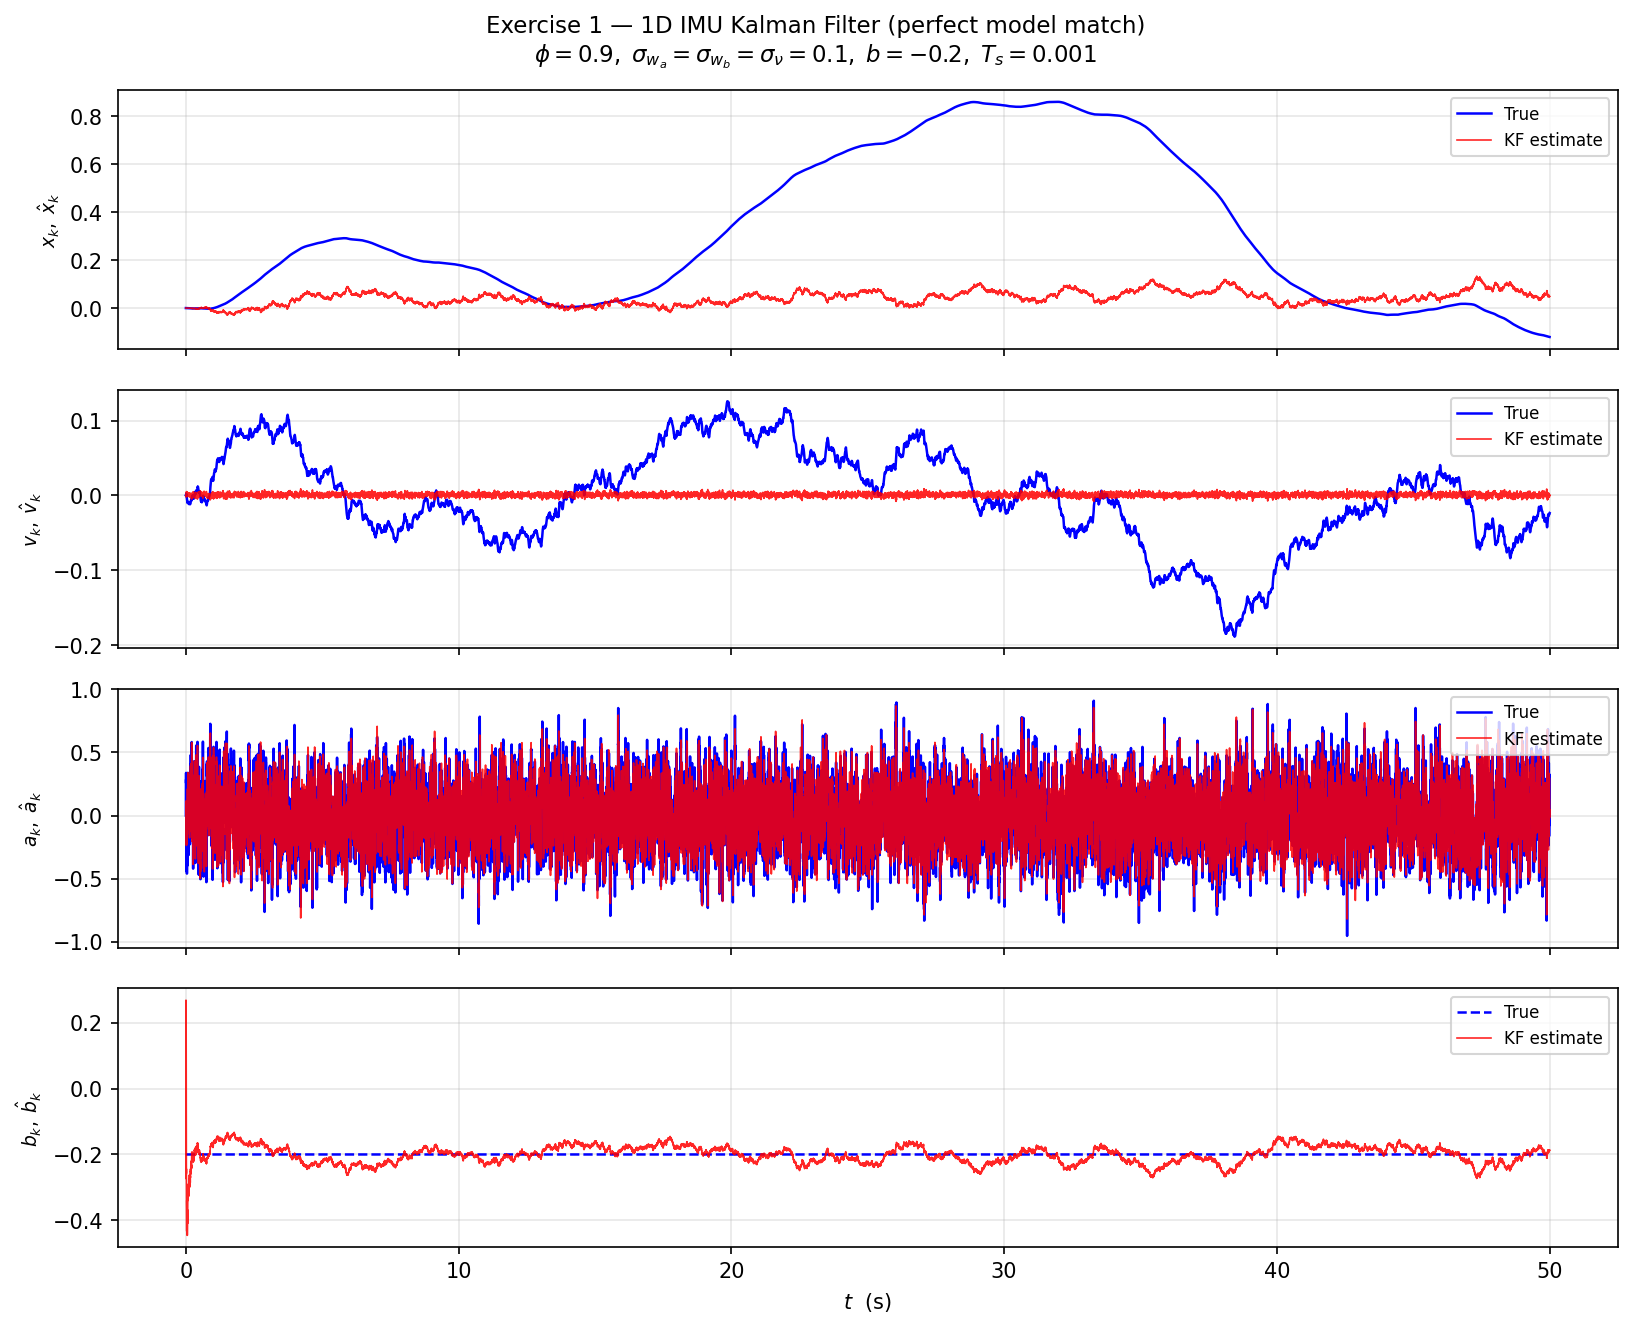
\includegraphics[width=\linewidth]{../../Exercises/Lecture_5/exercise1_sigma_wb_0001.png}
  \caption{$\sigma_{w_b} = 0.001$: bias estimate hovers around $-0.2$
           with small persistent oscillations.
           Because $Q_{33} = 10^{-6} > 0$, the covariance prediction
           re-inflates $P^{[b,b]}$ every step, keeping $K^{[b]}$
           non-zero and preventing the estimate from locking in.}
  \label{fig:sigmawb0001}
\end{figure}
\begin{figure}[H]
  \centering
  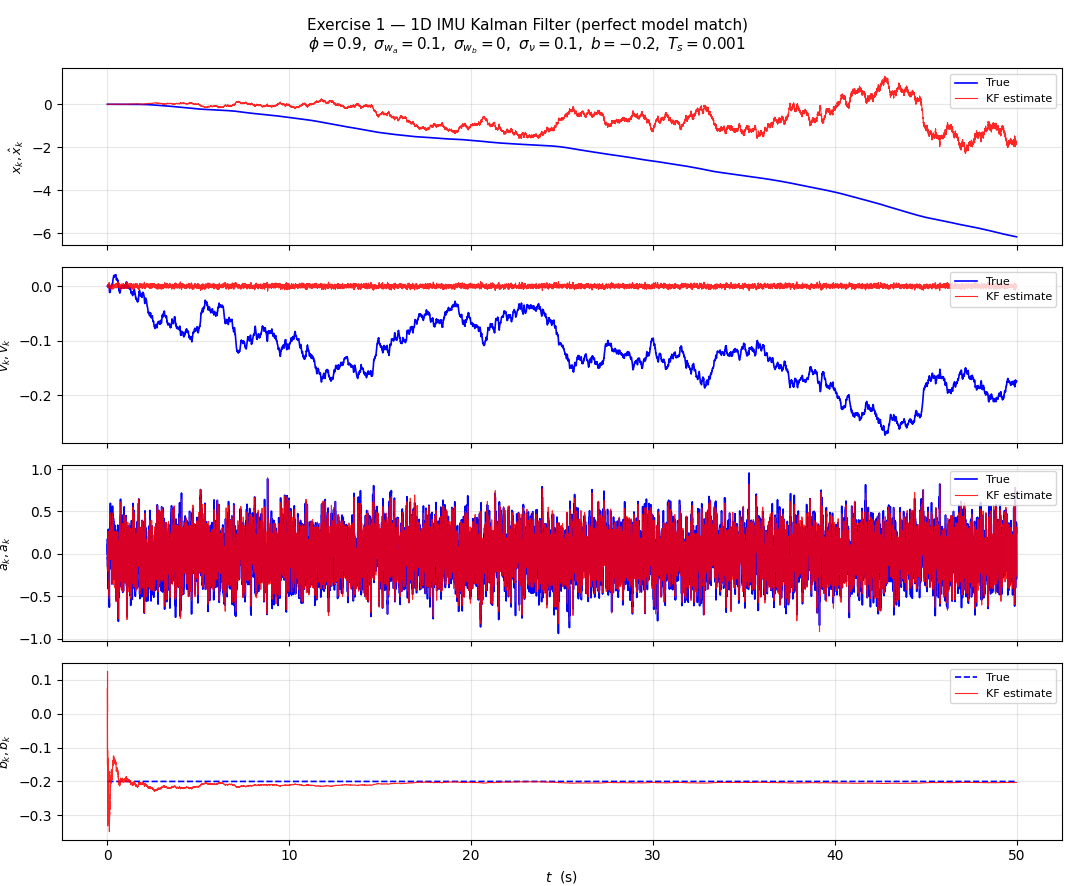
\includegraphics[width=\linewidth]{../../Exercises/Lecture_5/omega_wb=0.00.PNG}
  \caption{Python simulation output.
           \textbf{Blue} = true signal; \textbf{Red} = KF estimate.
           Parameters: $\phi=0.9$, $\sigma_{w_a}=\sigma_{w_b}=\sigma_\nu=0.0$,
           $b=-0.2$, $T_s=0.001$, $N=50\,000$ steps (50\,s).}
  \label{fig:sigmawb00}
\end{figure}

% ─────────────────────────────────────────────────────────────────────────────
\subsection*{Variable reference table}

\begin{center}
\renewcommand{\arraystretch}{1.5}
\begin{tabular}{p{2.8cm} p{2.0cm} p{8.5cm}}
  \toprule
  \textbf{Variable} & \textbf{Size} & \textbf{Meaning} \\
  \midrule
  $\boldsymbol{\chi}_k$
    & $4 \times 1$
    & True state vector $[x_k,\, v_k,\, a_k,\, b_k]^\top$ at time step $k$. \\
  $\hat{\boldsymbol{\chi}}_{k|j}$
    & $4 \times 1$
    & KF estimate of the state at step $k$, given all measurements up
      to step $j$.
      $j = k-1$: predicted (before new measurement);
      $j = k$: updated (after new measurement). \\
  $P_{k|j}$
    & $4 \times 4$
    & Error covariance matrix: the filter's uncertainty about
      $\hat{\boldsymbol{\chi}}_{k|j}$.
      Diagonal entries are the variance of each individual state
      estimate; off-diagonal entries capture correlations. \\
  $\boldsymbol{\Phi}$
    & $4 \times 4$
    & State transition matrix: maps the current state to the next
      state via the kinematic model ($x$, $v$) and the AR(1)/random-walk
      models ($a$, $b$). \\
  $Q$
    & $4 \times 4$
    & Process noise covariance: uncertainty added to the state at
      each prediction step.
      $Q_{33} = \sigma_{w_a}^2$ (acceleration noise);
      $Q_{44} = \sigma_{w_b}^2$ (bias drift noise);
      all other entries zero. \\
  $H$
    & $1 \times 4$
    & Measurement matrix: maps the state vector to the scalar
      measurement.
      $H = [0,0,1,1]$ picks out $a_k + b_k$ --- what the
      accelerometer reads. \\
  $R$
    & scalar
    & Measurement noise variance $\sigma_\nu^2$:
      how noisy a single accelerometer reading is. \\
  $y_k$
    & scalar
    & Accelerometer measurement at step $k$:
      $y_k = a_k + b_k + \nu_k$. \\
  $\tilde{y}_{k|k-1}$
    & scalar
    & Innovation: $y_k - H\hat{\boldsymbol{\chi}}_{k|k-1}$.
      How much the measurement differed from the filter's prediction.
      Zero means perfect prediction; large value means a surprising
      measurement. \\
  $S_k$
    & scalar
    & Innovation covariance: total uncertainty of the innovation,
      combining prediction uncertainty ($HP_{k|k-1}H^\top$) and
      sensor noise ($R$). \\
  $K_k$
    & $4 \times 1$
    & Kalman gain: optimal weight vector.
      Scales the innovation before adding it to each state.
      Small $K$ = trust prediction; large $K$ = trust measurement. \\
  $\phi$
    & scalar
    & AR(1) coefficient for the acceleration model ($= 0.9$).
      Controls how correlated consecutive acceleration values are:
      $\phi \to 1$ gives a random walk;
      $\phi \to 0$ gives uncorrelated white noise. \\
  $T_s$
    & scalar
    & Sample period in seconds ($= 0.001$\,s, i.e.\ 1\,kHz). \\
  $\sigma_{w_a}$
    & scalar
    & Standard deviation of the acceleration process noise per step
      ($= 0.1$). Controls how fast $a_k$ can change. \\
  $\sigma_{w_b}$
    & scalar
    & Standard deviation of the bias random-walk noise per step
      ($= 0.1$). Controls how fast $b_k$ can drift. \\
  $\sigma_\nu$
    & scalar
    & Standard deviation of the measurement (sensor) noise ($= 0.1$).
      $R = \sigma_\nu^2$. \\
  \bottomrule
\end{tabular}
\end{center}
% ==============================================================================
\clearpage
\begin{center}
\renewcommand{\arraystretch}{1.6}
\begin{tabular}{p{2.2cm} p{6cm} p{5.5cm}}
  \toprule
  \textbf{State} & \textbf{Observed behaviour} & \textbf{Why} \\
  \midrule
  Position $x_k$ &
    True signal drifts (random walk from double-integrating AR(1)
    acceleration).
    KF estimate stays near 0. &
    Position is unobservable: $H$ has zeros in column 1.
    No measurement anchors the position estimate. \\
  Velocity $v_k$ &
    Same --- true drifts, estimate stays near 0. &
    Velocity is also unobservable for the same reason. \\
  Acceleration $a_k$ &
    KF estimate closely tracks the true random signal. &
    $a_k$ appears directly in $y_k = a_k + b_k + \nu_k$;
    once bias is estimated the filter can recover $a$. \\
  Bias $b_k$ &
    Estimate starts at 0, converges to $-0.2$ within
    $\approx 10$\,s, then tracks the constant true bias. &
    Bias is also directly in the measurement.
    The KF separates $a$ from $b$ via their different dynamics
    (AR(1) vs.\ random walk) over the $\approx 10$\,s convergence
    time $1/(1-\phi)/T_s$. \\
  \bottomrule
\end{tabular}
\end{center}

\begin{warnbox}
  \textbf{Why does position diverge even with a ``perfect model match''?}\\
  ``Perfect model match'' means the filter's internal model is identical
  to the true system --- no mismatch.
  Yet position still drifts.
  This is an \textbf{observability} problem, not a modelling problem.\\[4pt]
  The only measurement is $y_k = a_k + b_k + \nu_k$.
  From this single signal, $a_k$ and $b_k$ can eventually be separated
  (via their dynamics), but $x_k$ and $v_k$ are simply not
  present in any measurement.
  To estimate position the system needs an external position sensor ---
  GPS, UWB, barometer, etc. --- adding a new row to $H$ and making
  $x_k$ observable.
\end{warnbox}

\begin{keybox}
  \textbf{Key takeaways --- Exercise 1}
  \begin{itemize}[leftmargin=1.4em, topsep=2pt]
    \item The KF recovers the unknown bias $b = -0.2$ from the raw
          accelerometer stream alone, within $\approx 10$\,s.
    \item Position and velocity diverge --- an \textbf{observability}
          problem, not a filter problem.
          Adding any absolute position sensor (GPS, UWB) would fix it.
    \item Bias random walk: zero-mean \emph{increments} but non-zero
          accumulated drift.
          The KF tracks the drift continuously at the cost of some
          residual noise in the bias estimate.
    \item Deterministic errors (scale factor, misalignment,
          g-sensitivity, temperature) are removed by pre-calibration
          (tumble test) and are not modelled here.
          Only the residual stochastic errors remain for the filter.
  \end{itemize}
\end{keybox}

% ==============================================================================
\begin{center}
\renewcommand{\arraystretch}{1.6}
\begin{tabular}{p{4.5cm} p{9.0cm}}
  \toprule
  \textbf{Syntax} & \textbf{What it does} \\
  \midrule
  \texttt{A @ B}
    & Matrix multiplication of \texttt{A} and \texttt{B}.
      Equivalent to \texttt{np.matmul(A, B)}.
      Works for 2-D arrays (matrix $\times$ matrix),
      2-D $\times$ 1-D (matrix $\times$ vector), and
      1-D $\times$ 1-D (dot product).
      Example: \texttt{H @ chi\_hat} multiplies the
      $(1\times4)$ matrix \texttt{H} by the $(4,)$ vector,
      giving a scalar. \\
  \texttt{np.eye(n)}
    & Returns the $n \times n$ \textbf{identity matrix} ---
      ones on the diagonal, zeros everywhere else.
      \texttt{np.eye(4)} gives the $4\times4$ identity used to
      initialise $P = I$ (``equal, moderate uncertainty in all
      states, no correlations''). \\
  \texttt{np.zeros(n)}
    & Returns a 1-D array of \texttt{n} zeros.
      \texttt{np.zeros(4)} gives \texttt{[0., 0., 0., 0.]} ---
      used to initialise \texttt{chi\_hat} (zero starting guess
      for all four states). \\
  \texttt{np.zeros(N)} (storage)
    & Same call, but used to pre-allocate an empty array of
      length $N$ to store results in the loop.
      Pre-allocating is faster than appending inside a loop. \\
  \texttt{np.diag([...])}
    & Creates a square \textbf{diagonal matrix} from a list.
      \texttt{np.diag([0, 0, 0.01, 0])} puts those values on
      the diagonal and zeros elsewhere --- used to build $Q$. \\
  \texttt{np.full(N, val)}
    & Returns an array of length $N$ where every entry is
      \texttt{val}.
      \texttt{np.full(N, -0.2)} creates the constant true-bias
      array for plotting. \\
  \texttt{np.random.randn()}
    & Draws \textbf{one} sample from $\mathcal{N}(0,1)$
      (standard normal: zero mean, unit variance). \\
  \texttt{np.random.randn(N)}
    & The argument \texttt{N} sets the \textbf{number of samples}
      returned --- gives a 1-D array of \texttt{N} independent
      draws from $\mathcal{N}(0,1)$.
      Used to generate all $N$ measurement noise samples at once
      rather than calling \texttt{randn()} inside the loop. \\
  \texttt{np.random.seed(s)}
    & Fixes the random number generator to seed \texttt{s} so
      the simulation produces the same random values every run.
      Remove or change \texttt{s} to get a different realization. \\
  \texttt{np.linalg.inv(A)}
    & Computes the \textbf{matrix inverse} $A^{-1}$.
      Used to compute $S_k^{-1}$ in the Kalman gain.
      For a scalar $S_k$ this is just $1/S_k$. \\
  \texttt{.flatten()}
    & Collapses any array to 1-D.
      After \texttt{K @ inn} the result can be shape $(4,1)$;
      \texttt{.flatten()} converts it to $(4,)$ so it can be
      added directly to \texttt{chi\_hat}. \\
  \texttt{.T}
    & \textbf{Transpose} of a 2-D array.
      \texttt{H.T} turns the $(1\times4)$ row vector into a
      $(4\times1)$ column vector. \\
  \bottomrule
\end{tabular}
\end{center}

% ==============================================================================
\clearpage
\section*{Exercise 2 \quad Acceleration as External Input (Slide 27)}

\subsection*{Exercise statement}

Implement the model with acceleration as a known external input (Slide~26)
and combine it with the Kalman filter using the same parameter values.
Replicate the figures on Slide~27.

\subsection*{Two-model approach}

This exercise uses \textbf{two different models} running in parallel ---
one for the true physical system and one inside the Kalman filter.

\medskip
\textbf{True system --- 3 states $[x,\,v,\,a]$ (Slide~26 model):}

Acceleration is a \emph{known} deterministic sinusoidal input
$a_k^{\text{input}}$, not a random state.
It is fed in via $\boldsymbol{\Gamma}$ and the $a$ row of
$\boldsymbol{\Phi}_{\text{true}}$ is zeroed so the input replaces it:

\[
\boldsymbol{\Phi}_{\text{true}} =
\begin{bmatrix} 1 & T_s & 0 \\ 0 & 1 & T_s \\ 0 & 0 & 0 \end{bmatrix},
\qquad
\boldsymbol{\Gamma} = \begin{bmatrix} 0 \\ 0 \\ 1 \end{bmatrix},
\qquad
\boldsymbol{\chi}_{\text{true},k} = \begin{bmatrix} x_k \\ v_k \\ a_k \end{bmatrix}
\]

\[
  \boldsymbol{\chi}_{\text{true},k+1}
  = \boldsymbol{\Phi}_{\text{true}}\,\boldsymbol{\chi}_{\text{true},k}
    + \boldsymbol{\Gamma}\,a_k^{\text{input}}
\]

The true bias $b = -0.2$ is a fixed constant added only in the measurement ---
it is not a state in the true system.

\medskip
\textbf{Kalman filter --- 4 states $[x,\,v,\,a,\,b]$ (Slide~23/25 model):}

The filter does \emph{not} know that acceleration is sinusoidal.
It uses the same Exercise~1 structure: acceleration modelled as an
AR(1) random process with $\phi = 0.9$.

\[
\boldsymbol{\Phi}_{\text{KF}} =
\begin{bmatrix}
  1 & T_s & 0    & 0 \\
  0 &  1  & T_s  & 0 \\
  0 &  0  & \phi & 0 \\
  0 &  0  & 0    & 1
\end{bmatrix},
\qquad
Q = \mathrm{diag}(0,\,0,\,\sigma_{w_a}^2,\,\sigma_{w_b}^2),
\qquad
H_{\text{KF}} = \begin{bmatrix} 0 & 0 & 1 & 1 \end{bmatrix}
\]

The filter sees only $y_k = a_k^{\text{input}} + b + \nu_k$ and must
separate the sinusoidal acceleration from the constant bias using only
the AR(1) model --- a \textbf{model mismatch}.

\begin{warnbox}
  \textbf{Why bias converges slowly and with persistent oscillations.}\\
  In Exercise~1 the true acceleration \emph{is} AR(1), so the filter
  model matches perfectly: the fast-varying part is cleanly attributed
  to $\hat{a}$ and the persistent offset to $\hat{b}$.\\[4pt]
  Here the true acceleration is a sinusoid with periods of 10\,s
  (0.1\,Hz) and 1\,s (1\,Hz), but the AR(1) model has a time constant
  of only $\tau = -T_s / \ln(\phi) \approx 10$\,ms.
  The model therefore expects acceleration to decorrelate in $\sim$10 steps,
  but the true sinusoidal components are correlated over thousands of steps.\\[4pt]
  The slow 0.1\,Hz sinusoid in particular looks almost
  like a slowly drifting bias to the AR(1) filter --- it cannot tell
  whether the gradual rise and fall is a changing bias or a very
  slow acceleration.
  Some of this sinusoidal variation leaks into $\hat{b}$, causing
  the bias estimate to overshoot at the start and then oscillate
  persistently around $-0.2$ rather than locking in cleanly.\\[4pt]
  In short: \textbf{the innovation always carries residual sinusoidal
  contamination that the AR(1) model cannot fully explain}, so a portion
  of it is continuously mis-attributed to the bias state.
\end{warnbox}

\subsection*{Acceleration input}

Two sinusoids are summed to create a realistic multi-frequency signal:
\[
  a_k^{\text{input}}
  = \sin(2\pi \cdot 0.1 \cdot t_k)
  + 0.7\,\sin(2\pi \cdot 1.0 \cdot t_k)
\]
The slow 0.1\,Hz component dominates the velocity and position drift;
the fast 1\,Hz component adds realistic high-frequency dynamics.

\subsection*{Results}

\begin{figure}[H]
  \centering
  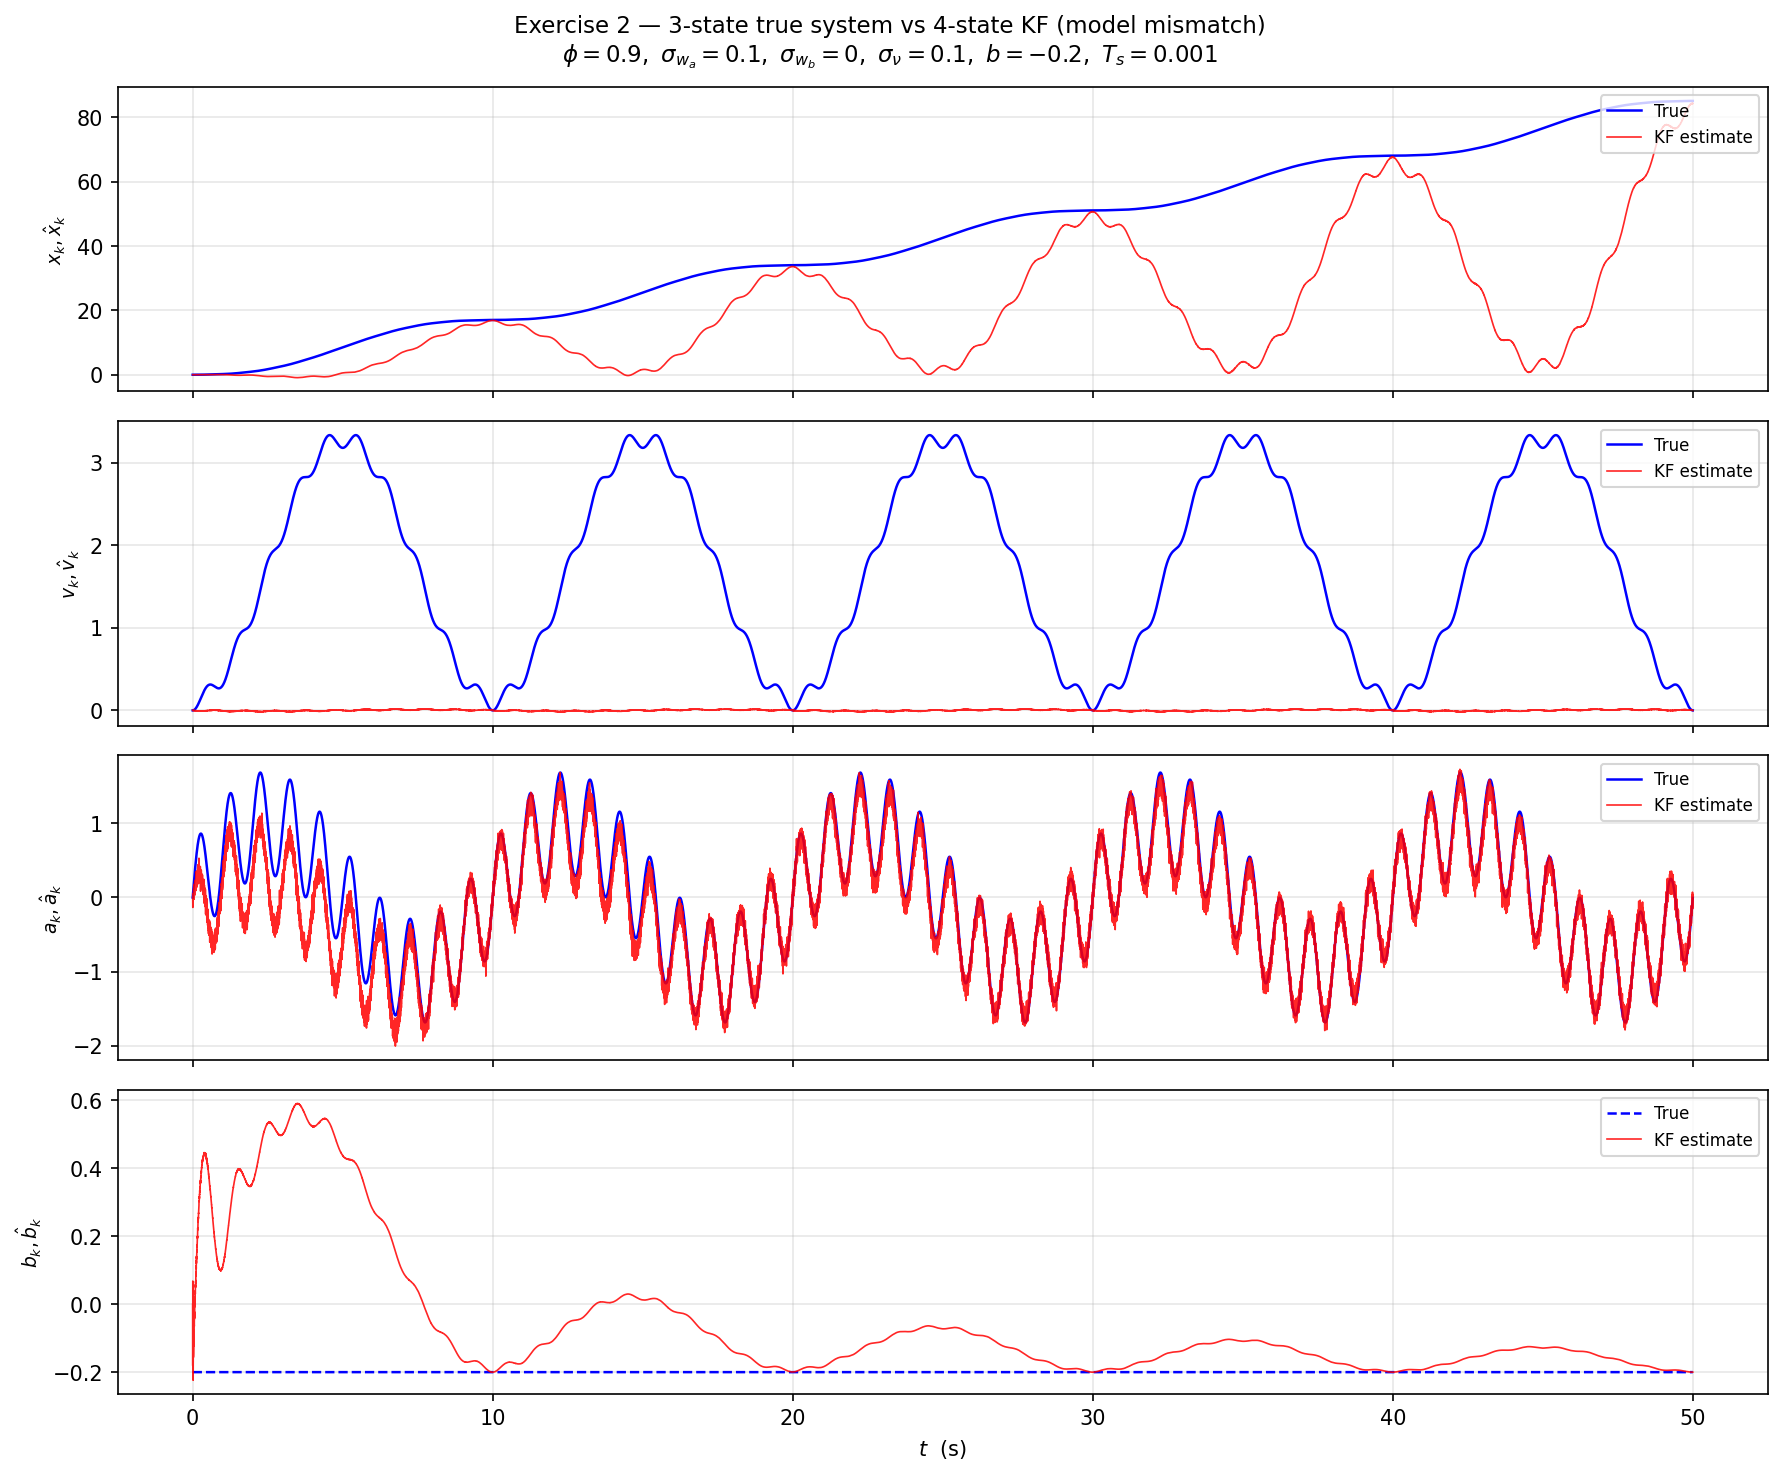
\includegraphics[width=\linewidth]{../../Exercises/Lecture_5/exercise2_slide27_replication.png}
  \caption{Exercise~2 simulation result.
           \textbf{Blue} = true signal; \textbf{Red} = KF estimate.
           True system: 3-state sinusoidal input model.
           KF: 4-state AR(1) estimator (model mismatch).}
  \label{fig:ex2result}
\end{figure}

\begin{center}
\renewcommand{\arraystretch}{1.5}
\begin{tabular}{p{2.2cm} p{5.5cm} p{6cm}}
  \toprule
  \textbf{State} & \textbf{Observed behaviour} & \textbf{Why} \\
  \midrule
  Position $x_k$ &
    True drifts to $\approx +80$; KF estimate diverges from truth. &
    $x$ is unobservable ($H$ has zeros in position column).
    KF prediction integrates $\hat{a}$, not the true input directly. \\
  Velocity $v_k$ &
    True oscillates with growing trend; estimate stays near 0. &
    Same observability problem --- $v$ not in measurement. \\
  Acceleration $a_k$ &
    True is the two-frequency sinusoid.
    KF estimate tracks reasonably but with some lag and error. &
    Model mismatch: KF uses AR(1) to estimate what is actually a
    deterministic sinusoid.
    The AR(1) model is flexible enough to partially track it. \\
  Bias $b_k$ &
    True flat at $-0.2$.
    Estimate starts at 0, overshoots, then converges within $\approx 10$\,s. &
    Despite the model mismatch on $a$, the filter still separates
    the persistent $-0.2$ offset from the faster-varying acceleration
    component. \\
  \bottomrule
\end{tabular}
\end{center}

\begin{notebox}
  \textbf{Model mismatch: AR(1) vs sinusoidal.}\\
  The KF thinks acceleration evolves as $a_{k+1} = \phi\,a_k + w_a$
  (stochastic, mean-reverting) but the truth is
  $a_k = \sin(\omega_1 t) + 0.7\sin(\omega_2 t)$ (deterministic, periodic).
  The AR(1) model with $\phi = 0.9$ has a time constant of
  $-T_s / \ln(\phi) \approx 10$\,ms --- fast enough to partially track
  the 0.1\,Hz slow component but not fast enough to cleanly follow
  the 1\,Hz component.
  The mismatch introduces persistent acceleration estimation error,
  which in turn contaminates the bias estimate during the transient.
  Once bias converges, the innovation becomes small and the filter settles.
\end{notebox}

\end{document}
